\documentclass{beamer}
\usepackage[utf8]{inputenc}

\usepackage[orientation=landscape,size=a0,scale=1.4,debug]{beamerposter}
\usepackage{hyperref}
\usetheme{Boadilla}
\usecolortheme{rose}

% biblatex (requires biber; sudo pacman -S biber)
\usepackage[style=authoryear-ibid]{biblatex} % biblatex
\addbibresource{"./content/bib/bib1.bib"}
\addbibresource{"./content/bib/bib2.bib"}

\usepackage{graphicx}
\graphicspath{ {./content/img/} }

\title[\href{https://nextgen.abdn.ac.uk}{NEXTGEN}]{\href{https://nextgen.abdn.ac.uk}{NEXTGEN}}
\subtitle{Neural Network Encryption: Exporation of Techniques for Secure Agricultural Data Processing}
\author[\href{https://nextgen.abdn.ac.uk}{nextgen.abdn.ac.uk} or \href{https://cryptolog.io}{cryptolog.io}]{\href{https://cryptolog.io}{George Onoufriou}, Paul Mayfield, Georgios Leontidis}
\date{\today}

\begin{document}

  \begin{frame}
    \maketitle
    \begin{columns}
      \begin{column}{0.3\textwidth}
        \begin{block}{Fully Homomorphic Encryption as a Service}
          Despite the ever increasing prevalence of monitoring, tracking, and sensing, generating more data than ever before, we currently are unable to process this data in many circumstances. In some industries and settings this inability to process data arises from the sensitivity or indeed perceived sensitivity of the data that would otherwise be required to train or make use of state-of-the-art deep learning models. Other scenarios where data could not be processed would also include a lack of expertise being available, in particular for smaller entities such as farms, start-ups, etc. \\
          We propose and show in practice how fully homomorphic encryption as a service (\ref{fig:pipeline}) can be used to both protect the privacy and security of data owners, while allowing third parties to be called upon for data processing itself without any ability to decrypt \autocite{gentry2009fully} and subsequently making it impossible for data to be compromised even by quantum decryption thanks to FHE using the ring learning with errors problem, instead of plain prime factorization in most non-FHE encryption.
        \end{block}
      \end{column}
      \begin{column}{0.35\textwidth}
        \begin{block}{Fully Homomorphically Encrypted Pipeline}
          \begin{figure}
            \centering
            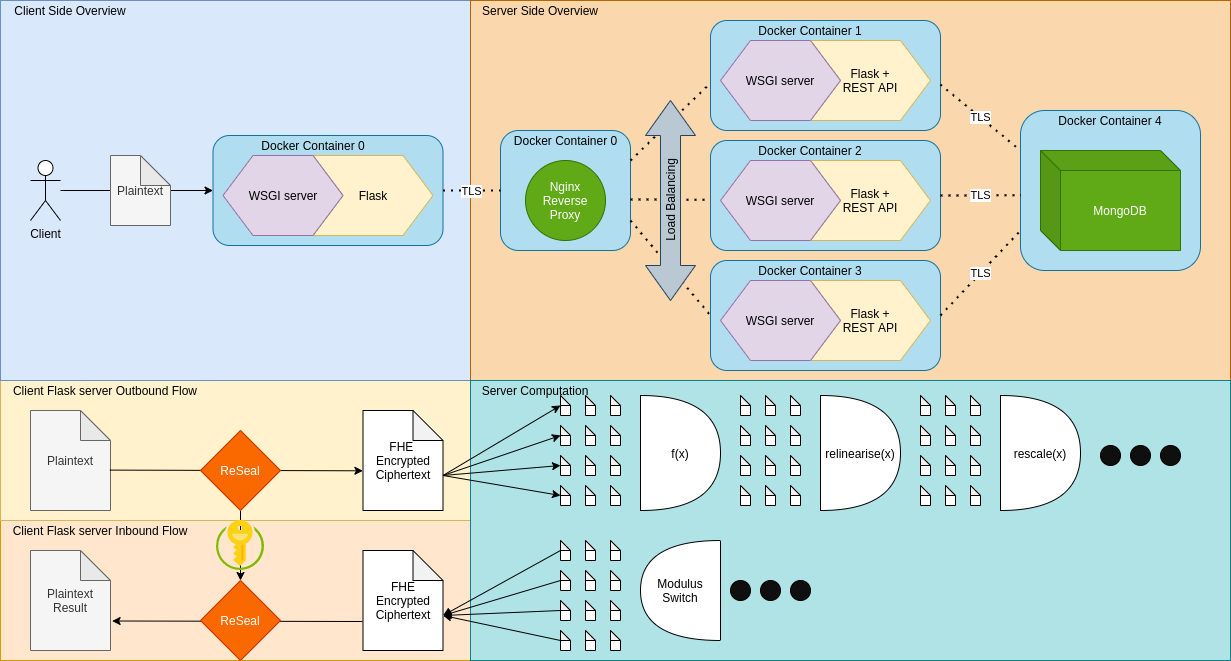
\includegraphics[width=\textwidth]{nextgen.png}
            \caption{Our server-client based pipeline and API for application and evaluation of FHE at some scale.}
            \label{fig:pipeline}
          \end{figure}
        \end{block}
      \end{column}
      \begin{column}{0.3\textwidth}
        \begin{block}{About our pipeline}
          To both evaluate, and implement FHE deep learning in practice, we decided to create a two part system:
          \begin{itemize}
            \item An on-site edge device server.
              \begin{itemize}
                \item The data encryptor, and key handler such that private keys have solely an on-site presence and thus are under the data owners direct control, and ultimately choice.
                \item Capable of edge compute for inference and prediction at the point of need without requiring any off-site processing.
                \item REST API for direct programmatic control and communication.
                \item Local web app for easy data submission and control for when there is limited time or expertise for fine grained API control.
                \item Serves as a gateway to our larger more powerful data processing backend, by sharing only ciphertexts without the respective private keys.
              \end{itemize}
            \item An off-site data processor.
              \begin{itemize}
                \item Higher performance hardware for much longer and more complex computations such as those in training.
                \item Configured and ready for scaling, with reverse proxies, and horizontal scalable MongoDB.
                \item REST API for scalable direct programmatic control and communication.
                \item Global web app for experimentation and testing.
                \item Can not decrypt any data since it will not have any private keys to decrypt with.
              \end{itemize}
          \end{itemize}
        \end{block}
      \end{column}
    \end{columns}

    \begin{columns}
      \begin{column}{0.6\textwidth}
        \begin{block}{Fully Homomorphic Encryption Compatible Simple 1D CNN Computational Graph}
          \begin{figure}
            \centering
            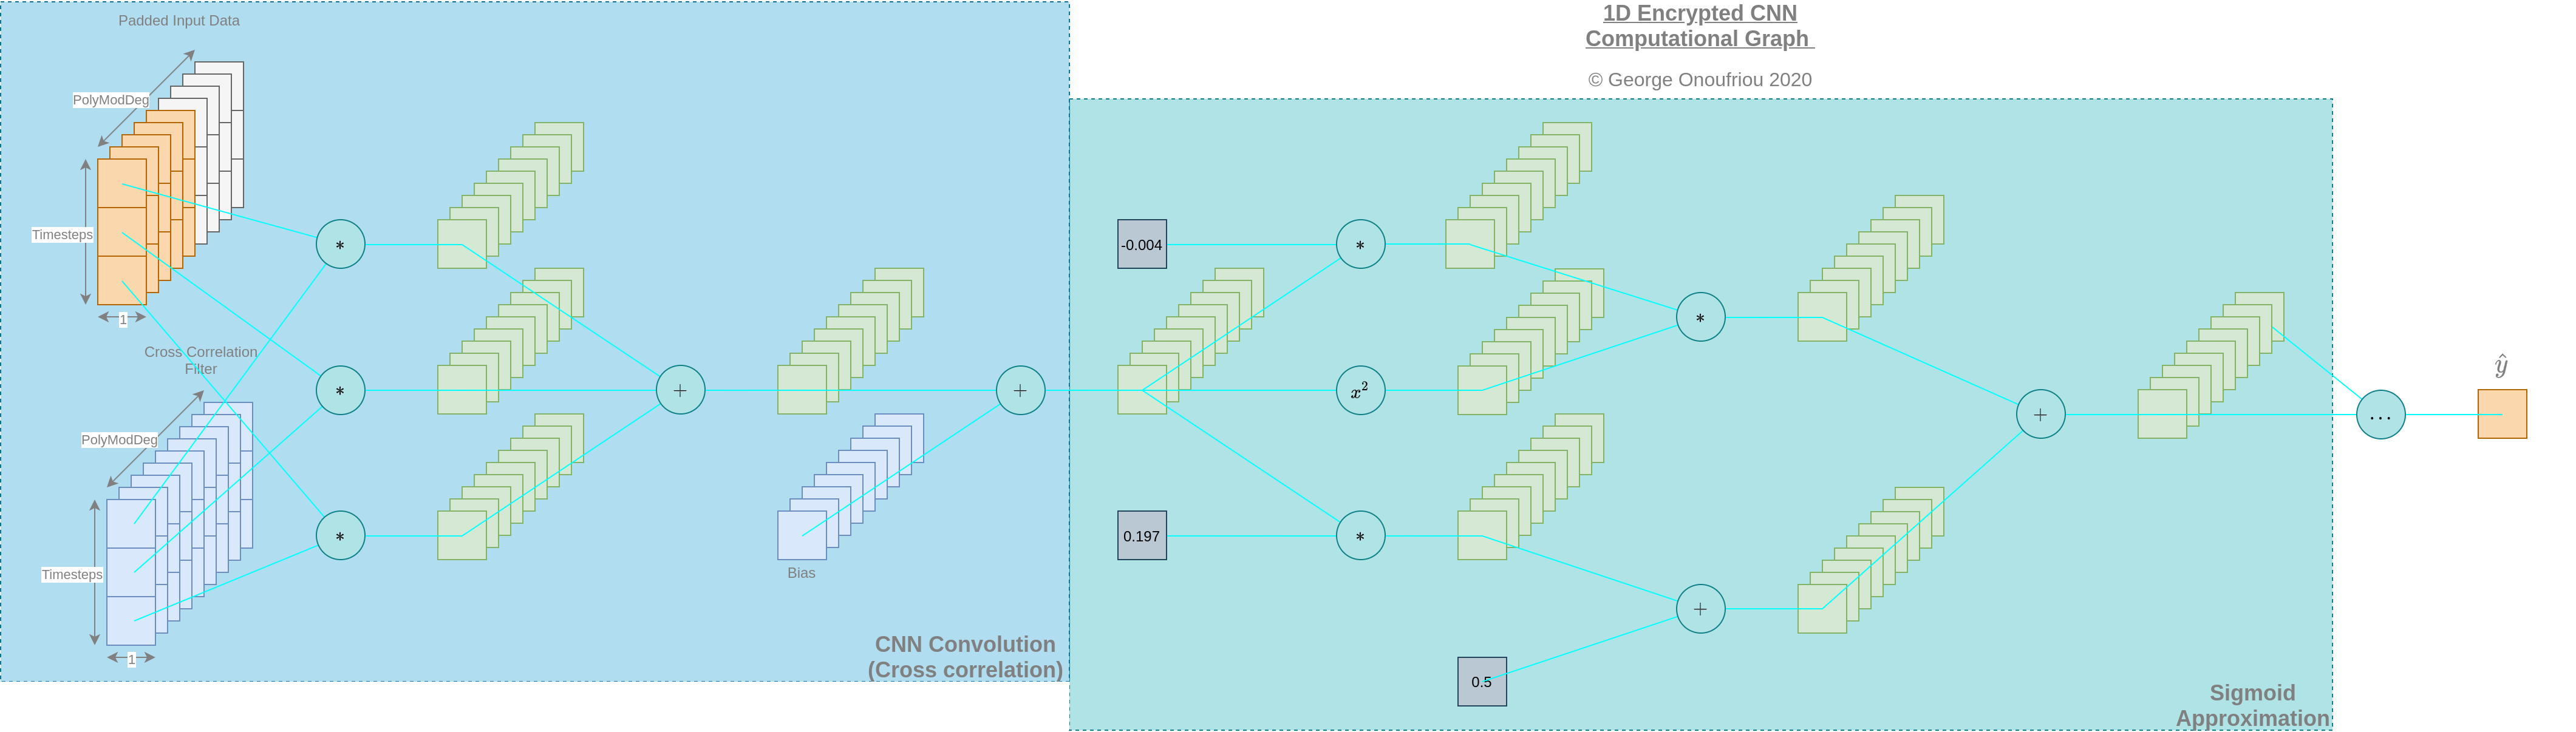
\includegraphics[width=\textwidth]{encrypted_cnn.png}
            \caption{FHE Compatible 1D CNN computational graph used to interchange space and time so historic milk yield and feeding cycles can be used to predict future yield while still using short computational depths of CNNs.}
            \label{fig:computational_graph}
          \end{figure}
        \end{block}
      \end{column}
      \begin{column}{0.35\textwidth}
        \begin{block}{Combining Deep Learning and Fully Homomorphic encryption}
          Deep learning is state-of-the-art and very pervasive in many machine learning tasks, such as time series prediction used here, thus we combine FHE with deep learning:
          \begin{itemize}
              \item Deep learning usually operates in the range 0-1 this we need to use the Cheon, Kim, Kim, and Song (CKKS) \autocite{ckks} encryption scheme which can use floating point numbers unlike most other schemes.
              \item Existing deep learning works predominantly exist in python, whereas most FHE libraries use C++, thus we created our own open-source bindings, and abstraction layer to take this C++ and integrate it with python and deep learning.
              \item Deep learning activation functions are usually incompatible with FHE since they require division such as sigmoid (Eq:\ref{sigmoid}).
              \item We use a polynomial sigmoid approximation (Eq:\ref{sigmoid_approx}) to avoid incompatibility.
              \item We use a 1D CNN in place of RNNs since the computational depth is shorter and wider.
              \item Shorter computational depth means we need less expensive operations to squish the ciphertext down (bootstrapping) to a manageable size.
              \item Wider more independent computations lend them selves better parallelization and optimization as they can occur simultaneously.
          \end{itemize}
        \end{block}
      \end{column}
    \end{columns}

    \begin{columns}
      \begin{column}{0.3\textwidth}
        \begin{block}{FHE Compatibility and Deep Learning Equation Summary}
          \begin{equation}
            \label{sigmoid}
            \sigma(x) = \frac{1}{1+e^{-x}}
          \end{equation}
          \begin{equation}
            \label{sigmoid_approx}
            \sigma(x) \approx 0.5 + 0.197x + -0.004x^3
          \end{equation}
          \begin{equation}
            \label{cnn_activation}
            a^{<t>}=\sigma(w_{i}^{<t>}x^{<t>}+b_i^{<t>})
          \end{equation}
          \begin{equation}
            \label{gradient}
            \frac{df}{d\sigma} = (1-\sigma(x)) * \sigma(x)
          \end{equation}
          \begin{equation}
            \label{weight_update}
            % learning rate
            w_i^{j+1<t>} = w_i^{j<t>} - (l * \frac{df}{dw_i^{j<t>}})
          \end{equation}
        \end{block}
      \end{column}
      \begin{column}{0.3\textwidth}
        \begin{block}{Future Work}
          This projects focus was on proving that FHE could be used in practice, and at some scale. However we have begun and would like to in future continue working on  solving problems such as:
          \begin{itemize}
            \item Training neural networks, including calculating gradients (Eq:\ref{gradient}), and weight updates while encrypted (Eq:\ref{weight_update}).
            \item Utilizing parallel compute on the GPU to accelerate computation.
            \item Improving on the efficiency and optimize FHE deep learning.
          \end{itemize}
        \end{block}
      \end{column}
      \begin{column}{0.3\textwidth}
        \begin{block}{References}
          \printbibliography
        \end{block}
      \end{column}
    \end{columns}
  \end{frame}
\end{document}
